\documentclass{llncs}
\usepackage{xcolor}
\usepackage[utf8]{inputenc}
\usepackage{amssymb}
\usepackage{amsmath}
\usepackage{tikz}
\usetikzlibrary{automata, positioning, arrows}
\tikzset{
->, % makes the edges directed
>=stealth, % makes the arrow heads bold
node distance=3cm, % specifies the minimum distance between two nodes. Change if necessary.
shorten >=1pt,
every state/.style={thick, fill=gray!10}, % sets the properties for each ’state’ node
inner sep=0pt,
minimum size=0pt,
initial text=$ $, % sets the text that appears on the start arrow
}

\begin{document}

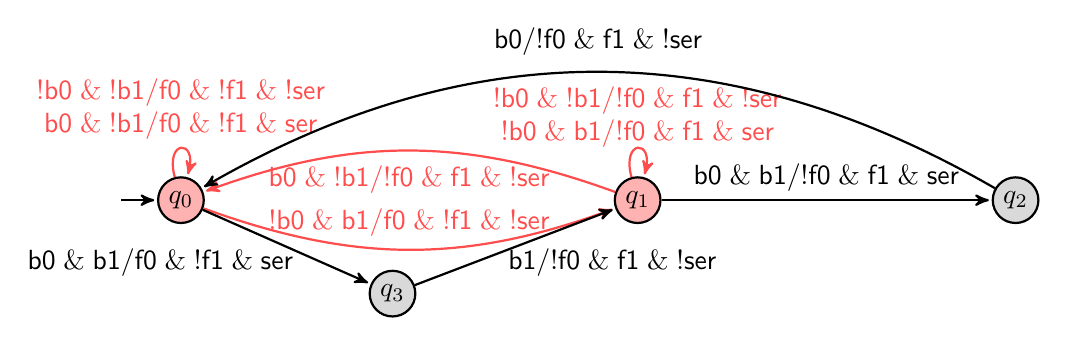
\begin{tikzpicture}[->,>=stealth',shorten >=1pt,auto,node distance=3.8cm,
                    thick,inner sep=0pt,minimum size=0pt]
  \tikzstyle{every state}=[fill=gray!30,text=black,inner
  sep=2pt,minimum size=12pt]

        \node[state, initial,fill=red!30] (q0) {$q_0$};
        \node[state, right of=q0, xshift=2cm,fill=red!30] (q1) {$q_1$};
        \node[state, right of=q1, xshift=1cm] (q2) {$q_2$};
        \node[state, below right of=q0, yshift=1.5cm] (q3) {$q_3$};
        \draw
            (q0) edge[loop above, align=center, color=red!70] node[yshift=1mm, color=red!70] {$!\mathsf{b0}\;\&\;!\mathsf{b1}/\mathsf{f0}\;\&\;!\mathsf{f1}\;\&\;!\mathsf{ser}$\\$\mathsf{b0}\;\&\;!\mathsf{b1}/\mathsf{f0}\;\&\;!\mathsf{f1}\;\&\;\mathsf{ser}$} (q0)
            (q0) edge[bend right=20, above, color=red!70] node[yshift=1.5mm, color=red!70]{$!\mathsf{b0}\;\&\;\mathsf{b1}/\mathsf{f0}\;\&\;!\mathsf{f1}\;\&\;!\mathsf{ser}$} (q1)
            (q0) edge[left] node[yshift=-2mm, xshift=1mm]{$\mathsf{b0}\;\&\;\mathsf{b1}/\mathsf{f0}\;\&\;!\mathsf{f1}\;\&\;\mathsf{ser}$} (q3)
            (q1) edge[loop above, align=center, color=red!70] node[color=red!70]{$!\mathsf{b0}\;\&\;!\mathsf{b1}/!\mathsf{f0}\;\&\;\mathsf{f1}\;\&\;!\mathsf{ser}$\\!$\mathsf{b0}\;\&\;\mathsf{b1}/!\mathsf{f0}\;\&\;\mathsf{f1}\;\&\;\mathsf{ser}$} (q1)
            (q1) edge[bend right=20, below, color=red!70] node[yshift=-1.7mm, color=red!70]{$\mathsf{b0}\;\&\;!\mathsf{b1}/!\mathsf{f0}\;\&\;\mathsf{f1}\;\&\;!\mathsf{ser}$} (q0)
            (q1) edge[above]
            node[yshift=1mm]{$\mathsf{b0}\;\&\;\mathsf{b1}/!\mathsf{f0}\;\&\;\mathsf{f1}\;\&\;\mathsf{ser}$} (q2)
            (q2) edge[bend right=30, above] node[yshift=2mm]{$\mathsf{b0}/!\mathsf{f0}\;\&\;\mathsf{f1}\;\&\;!\mathsf{ser}$} (q0)
            (q3) edge[right] node[yshift=-2mm, xshift=-1mm]{$\mathsf{b1}/!\mathsf{f0}\;\&\;\mathsf{f1}\;\&\;!\mathsf{ser}$} (q1);
    \end{tikzpicture}

\end{document}